\documentclass[a4paper]{report}
\pagestyle{headings}
\usepackage{hyperref}
\usepackage{listings}
\usepackage{graphicx}
\usepackage{hyperref}
\usepackage{color}
\lstset{language=bash}
\lstset{numbers=right}
\lstset{breaklines}
\title{Lab Report for Object-oriented Programming course \newline
 Lab 3: Linkage}
\author{Wang, Chen \\ 16307110064 \\ School of Software\\ Fudan University}
\date{\today}
\bibliographystyle{plain}
\begin{document}
\maketitle

\tableofcontents

\chapter{Understanding Internal and External Linkage}
\section{Requirements}
In this part, we are going to analyze the running result of the following short program and will try to make some subtle modifications whose change will result in the complete change of the result.
The codes are shown below.

\subsection{header.h}
\begin{lstlisting}[language=C++]
#ifndef LAB3_HEAER_H
#define LAB3_HEAER_H

static int variable = 0;
extern int variable2;
#endif //LAB3_HEAER_H

\end{lstlisting}


\subsection{file1.h}
\begin{lstlisting}[language=C++]
#ifndef LAB3_FILE1_H
#define LAB3_FILE1_H
void function1();

#endif //LAB3_FILE1_H

\end{lstlisting}

\subsection{file2.h}
\begin{lstlisting}[language=C++]
#ifndef LAB3_FILE2_H
#define LAB3_FILE2_H
void function2();

#endif //LAB3_FILE2_H

\end{lstlisting}


\subsection{file1.cpp}
\begin{lstlisting}[language=C++]
#include "header.h"

void function1() {
    variable = 1;
    variable2 = 1;
}
\end{lstlisting}

\subsection{file2.cpp}
\begin{lstlisting}[language=C++]
#include "header.h"
void function2() {
    variable = 2;
    variable2 = 2;

}
\end{lstlisting}

\subsection{main.cpp}
\begin{lstlisting}[language=C++]
#include <iostream>
#include "header.h"
#include "file1.h"
#include "file2.h"
int variable2;

int main() {
    function1();
    function2();

    std::cout << variable << std::endl;
    std::cout << variable2 << std::endl;
    return 0;
}
\end{lstlisting}



\section{Execution result}
The result of the execution is shown in the Figure \ref{1} below.

\begin{figure}
  \centering
  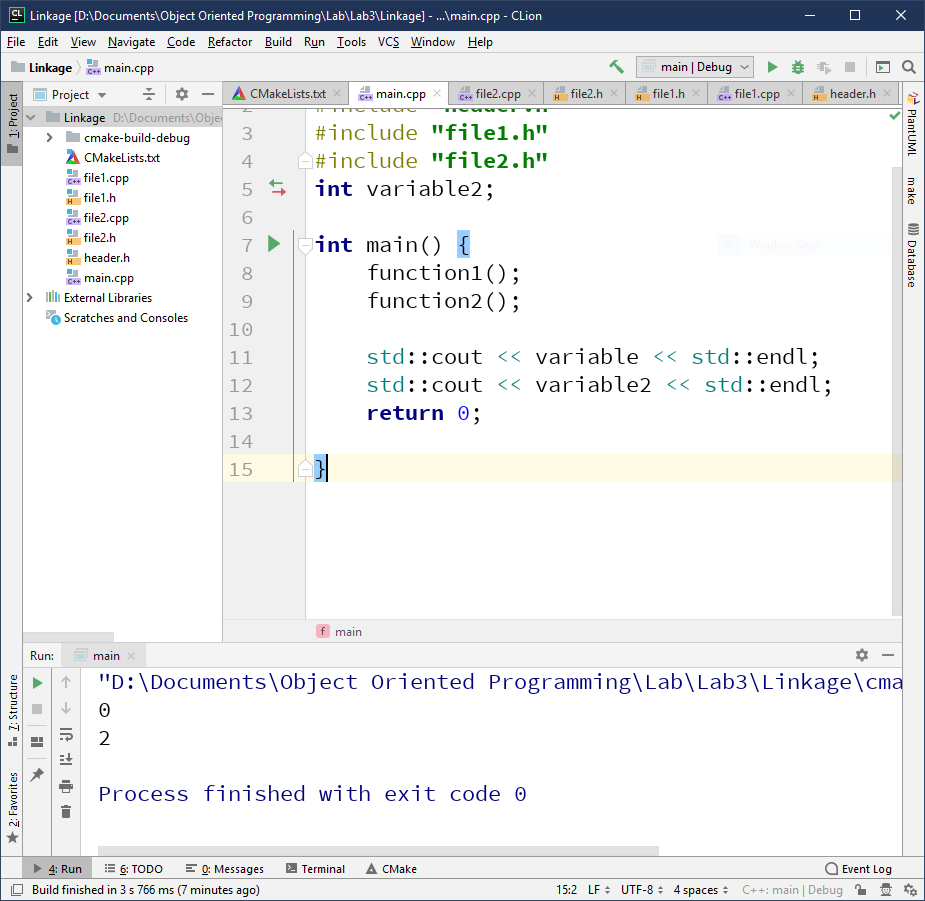
\includegraphics[scale=0.5]{result1.PNG}
  \caption{Execute Results}\label{1}
\end{figure}
\section{Analysis for the result of static variable}
From the C++ language standards, we can know that the \emph{static} keyword has different implications and effects in two different occasions. In this project, the keyword appears before the definition of the global variable outside from any methods. In this case, the \emph{static} keyword has the effect that the variable is only accessible in the specified file, i.e. having a \emph{file scope}.
\par
More specifically, in this project there are three \textbf{cpp} files in this project, each of them including the \emph{header.h} header file where a static variable is declared. In this case, each of the three files has a version of the static variable \emph{variable}. Therefore, the methods \emph{function1} and \emph{function2} will have no effect to the variable \emph{variable} in the \emph{main} method. Hence, the printing result is unchanged.

\section{Analysis for the result of global variable}
As to another part of this lab, the printing result of \emph{variable2}, is a typical example of a global variable. Nevertheless, one slightly point making the analysis more complex is that the \emph{external} keyword is used to make the global variable declared and defined at different places. 
\par
More specifically, in this project, the variable \emph{variable2} is declared in \emph{header.h} with an \emph{external} keyword, indicating that this variable will be defined somewhere else in this project. Then in the file \emph{main.cpp} this variable is defined. Therefore, this is a typical example of global variable and all the functions are modifying the same version of the variable. Therefore, the \emph{main} function will print the result after being changed in the other functions.

\section{Task 1.2: Duplicate variable definition}
The result of the change is shown in the Figure \ref{2} below, indicating an compiling error.


\begin{figure}
  \centering
  \includegraphics[scale=0.5]{Onetow.PNG}
  \caption{Execute Results of Task 1.2}\label{2}
\end{figure}


In this example, we have two places both defining the variable \emph{variable2}. Therefore, the compiler will report a duplicate definition error.
\section{Task 1.3: External declaration without definition}

The result of the change is shown in the Figure \ref{3} below, indicating an compiling error.


\begin{figure}
  \centering
  \includegraphics[scale=0.5]{Onethree.PNG}
  \caption{Execute Results of Task 1.3}\label{3}
\end{figure}


As per have stated above, an \emph{extern} keyword indicates that this variable is defined somewhere else in this file, hence it will cause a compiling error if no definition is made through out the project file.


\chapter{Understanding Name Space}
\section{Task 2.2 Duplicate variable naming in separate name spaces}
In this task, we are going to use the name space mechanism, create two variables with the same name but different values and print them.
\par
Here in my implementation, I declared two name spaces called \textbf{a} and \textbf{b} separately and then a variable named \textbf{a} in each name space but different value. Then in the \emph{main} method, these two variables are printed separately, we can see the result that they have different values printed. The result is shown in the Figure \ref{4} below.


\begin{figure}
  \centering
  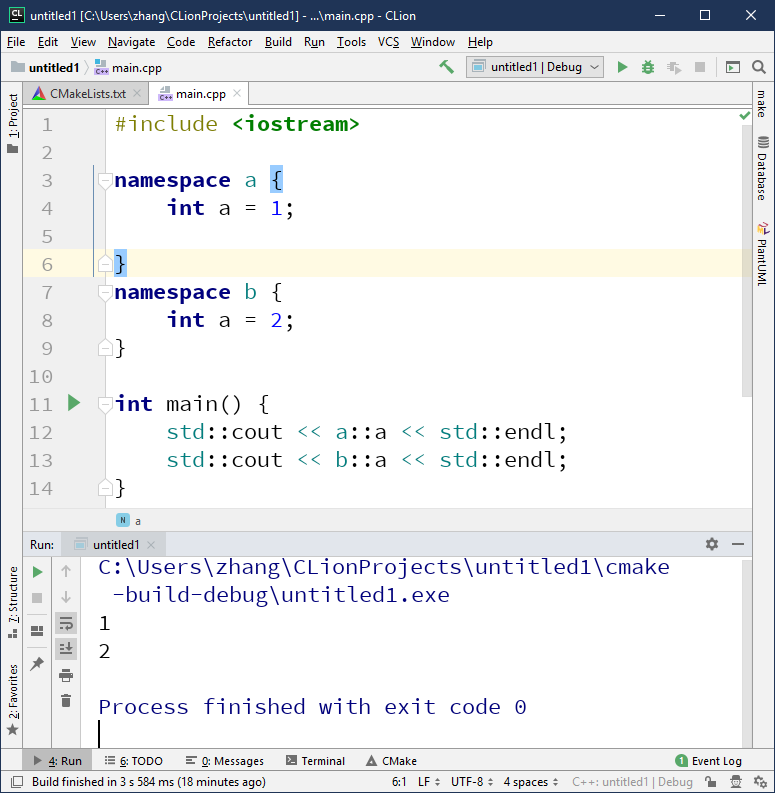
\includegraphics[scale=0.5]{TwoOne.PNG}
  \caption{Execute Results of Task 2.1}\label{4}
\end{figure}

\section{Task 2.2 Extended namespace}
In this task, I will need to duplicately declare the namespace of the same name in two files. The space of the first file defines ``ab=1; cd=2'', and the space of the second file is defined, ``ab=3;bc=4'' Finally, print the value in the namespace in the main function.
\par
Here in my implementation, I declared a name space called \textbf{a} in two separate files and then assigned different values to the variables as stated. Then in the \emph{main} method, these three variables are printed separately, we can see the result that this project cannot be compiled due to duplicate variable definition in the same name space. The result is shown in the Figure \ref{5} below.

\begin{figure}
  \centering
  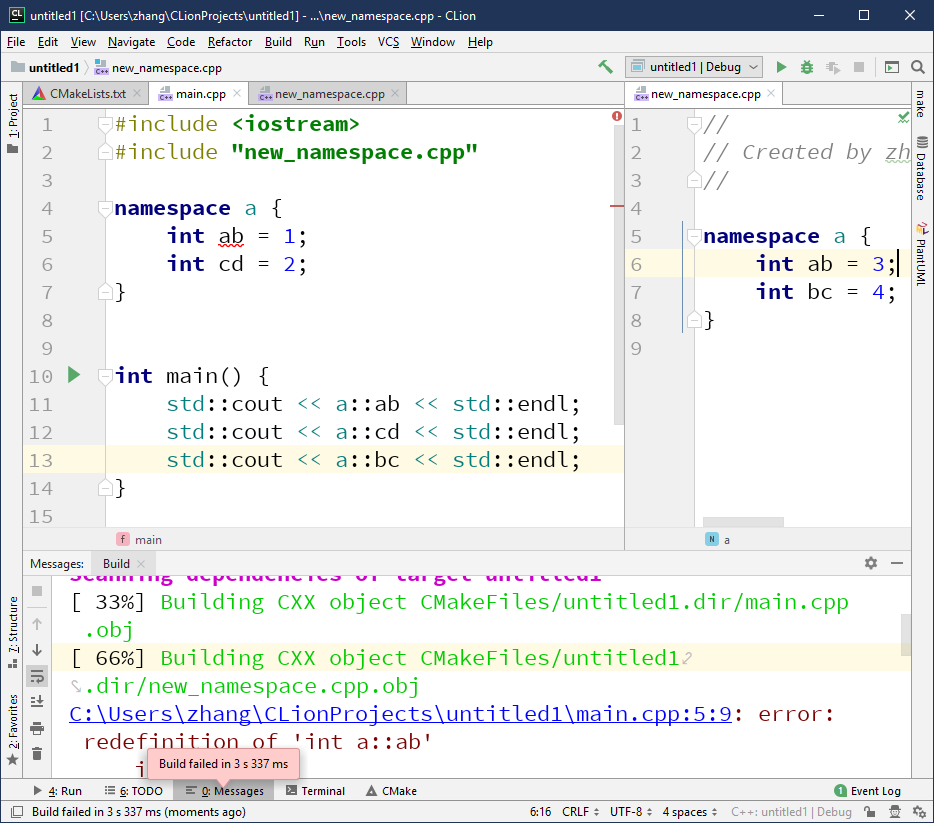
\includegraphics[scale=0.5]{TwoTwo.PNG}
  \caption{Execute Results of Task 2.2}\label{5}
\end{figure}

\chapter{Compare with Typescript Name Space}

\section{Modules in TypeScript}
\emph{\textbf{A note about terminology}: It’s important to note that in TypeScript 1.5, the nomenclature has changed. ``Internal modules'' are now ``namespaces''. ``External modules'' are now simply ``modules'', as to align with ECMAScript 2015\footnote{Ecma International. (2019, May 5). ECMAScript 2015 Language Specification – ECMA-262 6th Edition. In \emph{Ecma International}. Retrieved 08:23, May 11, 2019, from \url{http://www.ecma-international.org/ecma-262/6.0/}}'s terminology, (namely that \textcolor[rgb]{0.749,0.255,0.29}{module X \{ } is equivalent to the now-preferred \textcolor[rgb]{0.749,0.255,0.29}{namespace X \{} ).}
\subsection{Introduction}
Starting with ECMAScript 2015, JavaScript has a concept of modules. TypeScript shares this concept.
\par
Modules are executed within their own scope, not in the global scope; this means that variables, functions, classes, etc. declared in a module are not visible outside the module unless they are explicitly exported using one of the \emph{export} forms. Conversely, to consume a variable, function, class, interface, etc. exported from a different module, it has to be imported using one of the \emph{import} forms.
\par
Modules are declarative; the relationships between modules are specified in terms of imports and exports at the file level.
Modules import one another using a module loader. At runtime the module loader is responsible for locating and executing all dependencies of a module before executing it. Well-known modules loaders used in JavaScript are the CommonJS module loader for Node.js and require.js for Web applications.
\par
In TypeScript, just as in ECMAScript 2015, any file containing a top-level \emph{import} or \emph{export} is considered a module. Conversely, a file without any top-level \emph{import} or \emph{export} declarations is treated as a script whose contents are available in the global scope (and therefore to modules as well).
\subsection{Export}
\subsubsection{Exporting a declaration}
Any declaration (such as a variable, function, class, type alias, or interface) can be exported by adding the \emph{export} keyword.
\subsubsection{Export statements}
Export statements are handy when exports need to be renamed for consumers.
\subsubsection{Re-exports}
Often modules extend other modules, and partially expose some of their features. A re-export does not import it locally, or introduce a local variable.
\par
Optionally, a module can wrap one or more modules and combine all their exports using \emph{export * from ``module''} syntax.
\subsection{Import}
Importing is just about as easy as exporting from a module. Importing an exported declaration is done through using one of the \emph{import} forms below:

\begin{enumerate}
\item Import a single export from a module
\item Import the entire module into a single variable, and use it to access the module exports
\item Import a module for side-effects only
\end{enumerate}

Though not recommended practice, some modules set up some global state that can be used by other modules. These modules may not have any exports, or the consumer is not interested in any of their exports.
\subsection{Default exports}
Each module can optionally export a \emph{default} export. Default exports are marked with the keyword \emph{default}; and there can only be one \emph{default} export per module. \emph{default} exports are imported using a different import form.
\emph{default} exports are really handy. For instance, a library like jQuery might have a default export of \emph{jQuery} or \$, which we’d probably also import under the name \$ or jQuery.
\par
Classes and function declarations can be authored directly as default exports. Default export class and function declaration names are optional.
\subsection{\emph{export =} and \emph{import = require()}}
Both CommonJS and AMD generally have the concept of an \emph{exports} object which contains all exports from a module.
\par
They also support replacing the \emph{exports} object with a custom single object. Default exports are meant to act as a replacement for this behavior; however, the two are incompatible. TypeScript supports \emph{export =} to model the traditional CommonJS and AMD workflow.
\par
The \emph{export =} syntax specifies a single object that is exported from the module. This can be a class, interface, namespace, function, or enum.
\par
When exporting a module using \emph{export =}, TypeScript-specific \emph{import module = require("module")} must be used to import the module.

\subsection{Code Generation for Modules}
Depending on the module target specified during compilation, the compiler will generate appropriate code for Node.js (\textbf{CommonJS}), require.js (\textbf{AMD}), \textbf{UMD}, \textbf{SystemJS}, or \textbf{ECMAScript 2015 native modules} (ES6) module-loading systems. 

\subsection{Optional Module Loading and Other Advanced Loading Scenarios}
In some cases, you may want to only load a module under some conditions. In TypeScript, we can use the pattern shown below to implement this and other advanced loading scenarios to directly invoke the module loaders without losing type safety.
\par
The compiler detects whether each module is used in the emitted JavaScript. If a module identifier is only ever used as part of a type annotations and never as an expression, then no \emph{require} call is emitted for that module. This elision of unused references is a good performance optimization, and also allows for optional loading of those modules.
The core idea of the pattern is that the \emph{import id = require("...")} statement gives us access to the types exposed by the module. The module loader is invoked (through \emph{require}) dynamically, as shown in the if blocks below. This leverages the reference-elision optimization so that the module is only loaded when needed. For this pattern to work, it’s important that the symbol defined via an \emph{import} is only used in type positions (i.e. never in a position that would be emitted into the JavaScript).
To maintain type safety, we can use the \emph{typeof} keyword. The \emph{typeof} keyword, when used in a type position, produces the type of a value, in this case the type of the module.

\section{Name space in TypeScript}
\subsection{Introduction}
In this subsection I will try to outline the various ways to organize the code using namespaces (previously “internal modules”) in TypeScript. As per alluded in previous section's note about terminology, ``internal modules'' are now referred to as “namespaces”. Additionally, anywhere the module keyword was used when declaring an internal module, the namespace keyword can and should be used instead. This avoids confusing new users by overloading them with similarly named terms.
\subsection{Namespacing}
As we have more and more methods of the same or of similiar functions, we're going to want to have some kind of organization scheme so that we can keep track of our types and not worry about name collisions with other objects. Instead of putting lots of different names into the global namespace, we can wrap up our objects into a namespace.
\par
If we want the interfaces and classes in the namespace to be visible outside the namespace, we can preface them with export. Conversely, the implementation details can be left unexported and will not be visible to code outside the namespace. 
\subsection{Splitting Across Files}
As our application grows, we’ll want to split the code across multiple files to make it easier to maintain.
\subsubsection{Multi-file namespaces}
We can split our namespace across many files. Even though the files are separate, they can each contribute to the same namespace and can be consumed as if they were all defined in one place. Because there are dependencies between files, we’ll add reference tags to tell the compiler about the relationships between the files.
\subsection{Aliases}
Another way that you can simplify working with namespaces is to use \emph{import q = x.y.z} to create shorter names for commonly-used objects. Not to be confused with the \emph{import x = require("name")} syntax used to load modules, this syntax simply creates an alias for the specified symbol. We can use these sorts of imports (commonly referred to as aliases) for any kind of identifier, including objects created from module imports.
\par
Notice that we don’t use the \emph{require} keyword; instead we assign directly from the qualified name of the symbol we’re importing. This is similar to using \emph{var}, but also works on the type and namespace meanings of the imported symbol. Importantly, for values, \emph{import} is a distinct reference from the original symbol, so changes to an aliased \emph{var} will not be reflected in the original variable.

\section{Difference and relation between modules and name spaces in TypeScript}
\subsection{Introduction}
In this section, I will try to  clarify the difference on both concept and usage of modules and namespace in Typescript.
\subsection{Using Namespaces}
Namespaces are simply named JavaScript objects in the global namespace. This makes namespaces a very simple construct to use. They can span multiple files, and can be concatenated using \emph{--outFile}. Namespaces can be a good way to structure your code in a Web Application, with all dependencies included as \emph{<script>} tags in your HTML page.
\par
Just like all global namespace pollution, it can be hard to identify component dependencies, especially in a large application.
\subsection{Using Modules}
Just like namespaces, modules can contain both code and declarations. The main difference is that modules \textbf{declare} their dependencies.
\par
Modules also have a dependency on a module loader (such as CommonJs/Require.js). For a small JS application this might not be optimal, but for larger applications, the cost comes with long term modularity and maintainability benefits. Modules provide for better code reuse, stronger isolation and better tooling support for bundling.
\par
It is also worth noting that, for Node.js applications, modules are the default and the recommended approach to structure your code.
\par
Starting with ECMAScript 2015, modules are native part of the language, and should be supported by all compliant engine implementations. Thus, for new projects modules would be the recommended code organization mechanism.
\section{Internal Linkage in C}
If the declaration of a file-scope identifier for an object or a function contains the \textbf{storage-class-specifier} \emph{static}, the identifier has internal linkage. Otherwise, the identifier has external linkage. 
\par
Within one translation unit, each instance of an identifier with internal linkage denotes the same identifier or function. Internally linked identifiers are unique to a translation unit.
\section{External Linkage in C}
If the first declaration at file-scope level for an identifier does not use the \emph{static} storage-class specifier, the object has external linkage.
\par
If the declaration of an identifier for a function has no \textbf{storage-class-specifier}, its linkage is determined exactly as if it were declared with the \textbf{storage-class-specifier} \emph{extern}. If the declaration of an identifier for an object has file scope and no \textbf{storage-class-specifier}, its linkage is external.
An identifier's name with external linkage designates the same function or data object as does any other declaration for the same name with external linkage. The two declarations can be in the same translation unit or in different translation units. If the object or function also has global lifetime, the object or function is shared by the entire program.
\section{Name space in C++}
\subsection{Introduction}
A namespace is a declarative region that provides a scope to the identifiers (the names of types, functions, variables, etc) inside it. Namespaces are used to organize code into logical groups and to prevent name collisions that can occur especially when your code base includes multiple libraries. All identifiers at namespace scope are visible to one another without qualification. Identifiers outside the namespace can access the members by using the fully qualified name for each identifier, for example \emph{std::vector<std::string> vec;}, or else by a using Declaration for a single identifier (\emph{using std::string}), or a using Directive for all the identifiers in the namespace (\emph{using namespace std;}). Code in header files should always use the fully qualified namespace name.
\subsection{\emph{using} directives}
The \emph{using} directive allows all the names in a \emph{namespace} to be used without the \textbf{namespace-name} as an explicit qualifier. Use a using directive in an implementation file (i.e. *.cpp) if you are using several different identifiers in a namespace; if you are just using one or two identifiers, then consider a using declaration to only bring those identifiers into scope and not all the identifiers in the namespace. If a local variable has the same name as a namespace variable, the namespace variable is hidden. It is an error to have a namespace variable with the same name as a global variable.
\subsection{Declaring namespaces and namespace members}
Typically, you declare a namespace in a header file. If your function implementations are in a separate file, then qualify the function names.
\par
A namespace can be declared in multiple blocks in a single file, and in multiple files. The compiler joins the parts together during preprocessing and the resulting namespace contains all the members declared in all the parts. An example of this is the std namespace which is declared in each of the header files in the standard library.
\par
Members of a named namespace can be defined outside the namespace in which they are declared by explicit qualification of the name being defined. However, the definition must appear after the point of declaration in a namespace that encloses the declaration's namespace.
\subsection{The global namespace}
If an identifier is not declared in an explicit namespace, it is part of the implicit global namespace. In general, try to avoid making declarations at global scope when possible, except for the entry point main Function, which is required to be in the global namespace. To explicitly qualify a global identifier, use the scope resolution operator with no name, as in \emph{::SomeFunction(x);}. This will differentiate the identifier from anything with the same name in any other namespace, and it will also help to make your code easier for others to understand.
\subsection{The std namespace}
All C++ standard library types and functions are declared in the \emph{std} namespace or namespaces nested inside \emph{std}.
\subsection{Nested namespaces}
Namespaces may be nested. An ordinary nested namespace has unqualified access to its parent’s members, but the parent members do not have unqualified access to the nested namespace (unless it is declared as inline).
\par
Ordinary nested namespaces can be used to encapsulate internal implementation details that are not part of the public interface of the parent namespace.
\subsection{Inline namespaces (C++ 11)}
In contrast to an ordinary nested namespace, members of an inline namespace are treated as members of the parent namespace. This characteristic enables argument dependent lookup on overloaded functions to work on functions that have overloads in a parent and a nested inline namespace. It also enables you to declare a specialization in a parent namespace for a template that is declared in the inline namespace.
\par
You can use inline namespaces as a versioning mechanism to manage changes to the public interface of a library. For example, you can create a single parent namespace, and encapsulate each version of the interface in its own namespace nested inside the parent. The namespace that holds the most recent or preferred version is qualified as inline, and is therefore exposed as if it were a direct member of the parent namespace. Client code that invokes the Parent::Class will automatically bind to the new code. Clients that prefer to use the older version can still access it by using the fully qualified path to the nested namespace that has that code.
\par
The inline keyword must be applied to the first declaration of the namespace in a compilation unit.
\subsection{Namespace aliases}
Namespace names need to be unique, which means that often they should not be too short. If the length of a name makes code difficult to read, or is tedious to type in a header file where using directives can’t be used, then you can make a namespace alias which serves as an abbreviation for the actual name.
\section{Difference and relation between TypeScript module and C++ internal linkage}
There is no obvious relationship between module in TypeScript and internal linkage in C++. Nevertheless, the usage of internal linkage has something similar to the variables defined inside a module in TypeScript. 
\par
An internal linking variable in C++ has its scope inside the file or the translation unit; while any variable inside a module in TypeScript has its scope inside this module and invisible to any member outside the module unless they are explicitly using one of the \emph{export} forms. Hence this indicates both the similarity and the difference between a module in TypeScript and internal linkage in C++: both are visible to the specified scope while a variable in a module in TypeScript can be explicitly exported while an internal linking variable in C++ can never be exported again.
\section{Difference and relation between TypeScript module and C++ external linkage}
As stated in the previous section above, we can see the similarity and difference between the module in TypeScript and external linkage in C++. The module itself has nothing to do with the external linkage in C++ while the variables in a module in TypeScript can have similar behavior as the external linking variables in C++. 
\par
The external linkage makes use of the variables defined somewhere else; similarly, when importing an module, we are also utilizing the variables defined somewhere else. However, there are still several distinct differences between the external linkage and the module import. As have been described in the several previous sections, importation in TypeScript can  have several forms and could be used in freedom at a rather large scale. That is, we can specify whether we want to import a variable, a function, or several of them or the entire module. We can also specify any one of them an alias when importing, while in C++ we can only link one function or variable at a time, unable to change the name of it.
\section{Difference and relation between TypeScript module and C++ name space}
A module has great similarity with C++ name space -- they are designed with the same purpose, actually. Both of them are designed to cope with the problem of naming conflict. Both variables in a module and variables in a name space could be accessed via the corresponding module or name space. 
\par
However, they have some more distinctions in detail. 
\begin{enumerate}
\item Each module in TypeScript is at file level. That is, any file containing a top-level \emph{import} or \emph{export} is considered a module. Conversely, any file without a top-level \emph{import} or \emph{export} is not a module. However, in C++, name space does not have to have relationship with file. In a file, there can be several name spaces without interacting with each other. 
\item
In C++, name space has a weak relationship with files, that is, they are actually decoupled from each other. Any file can declare using any name space. When including files, the compiler will not care about which name space the file is using. And we can call functions by addressing their name space without importing any specific name space. However, in TypeScript, a  module is coupled with a file and a file with \emph{import} or \emph{export} is a module. Since there is no including directive in TypeScript, importing an module is the process of importing an file. In addition, we can specify what contents the import and what alias we want to use.
\item
Unlike C++, where during the process of importing, all the contents of the imported file are copied into the destination, TypeScript can choose what contents to import and what to be left.
\item
In TypeScript, there is the mechanism of a \emph{default export}, where such mechanism is missing in C++. However, it is not needed because C++ importing allows everything accessible.
\end{enumerate}
\par

\section{Difference and relation between TypeScript name space and C++ internal linkage}
Just like the relationship between TypeScript module and C++ internal linkage, TypeScript name space and C++ internal linkage are two different objects but the variables inside a TypeScript name space and the variables declared with internal linkage has something in common.
\par
A variable defined inside a TypeScript can only be accessed inside the name space so as to avoid collision, and the internal linking variables are accessible in its scope. However, there are some distinctions between the scopes of the two things. A name space can go across various files and the functions and variables can be exported towards outside the name space. Nevertheless, in C++ internal linkage, the scope is strictly defined to be inside the translation unit and no more addition modifier is allowed.
\section{Difference and relation between TypeScript name space and C++ external linkage}
Just like the relationship between TypeScript module and C++ external linkage, TypeScript name space and C++ external linkage are two different objects but the variables inside a TypeScript name space and the variables declared with external linkage has something in common.
\par
Variables inside a name space in TypeScript can be shared and accessible to the codes with the same name space, or exported so that can be used in other name spaces. However, in C++, the variables only need to be declared to be \emph{external} variables and then it can be used if it is actually defined somewhere else. 
\section{Difference and relation between TypeScript name space and C++ name space}
The name space in TypeScript and name space in C++ have great in common, especially from the perspectives of purpose of design and functions. Therefore, the similarity of TypeScript name space and the C++ name space is omitted here and only differences are mentioned.
\par
In TypeScript name space, visibility mechanism is utilized so that developers can choose what are visible to the codes outside the name space and what are visible. However, in C++ everything in a name space is visible to the codes declaring using the same name space.

\begin{thebibliography}{A}
\bibitem{1}
Wikipedia contributors. (2019, May 5). TypeScript. In \emph{Wikipedia, The Free Encyclopedia}. Retrieved 08:23, May 11, 2019, from \url{https://en.wikipedia.org/w/index.php?title=TypeScript&oldid=895568490}

\bibitem{2}
Wikipedia contributors. (2019, May 9). JavaScript. In \emph{Wikipedia, The Free Encyclopedia}. Retrieved 08:24, May 11, 2019, from \url{https://en.wikipedia.org/w/index.php?title=JavaScript&oldid=896215789}

\bibitem{3}
Wikipedia contributors. (2019, April 24). C++. In \emph{Wikipedia, The Free Encyclopedia}. Retrieved 08:25, May 11, 2019, from \url{https://en.wikipedia.org/w/index.php?title=C%2B%2B&oldid=893975016}

\bibitem{4}
Wikipedia contributors. (2019, February 27). Object-oriented programming. In \emph{Wikipedia, The Free Encyclopedia}. Retrieved 10:22, March 23, 2019, from \url{https://en.wikipedia.org/w/index.php?title=Object-oriented_programming&oldid=885274966}

\bibitem{5}
Wikipedia contributors. (2019, March 18). Namespace. In \emph{Wikipedia, The Free Encyclopedia}. Retrieved 08:27, May 11, 2019, from \url{https://en.wikipedia.org/w/index.php?title=Namespace&oldid=888324103}
\end{thebibliography}
\end{document} 